% REFERENCIAL TEORICO----------------------------------------------------------

\chapter{REFERÊNCIAL TEÓRICO}
\label{chap:ref-teorico}

% \section{Computação de Alto Desempenho}
\section{Programação Paralela}

Um programa de processamento paralelo é um único programa que é executado em vários processadores simultaneamente.
A programação paralela pode ser usada para o reduzir o tempo de execução de um programa,
que busca encontrar uma solução para um problema complexo, como por exemplo, problemas voltados as áreas científicas \cite{hennessy2014organizaccao}.

A diferença de um programa sequencial para um programa paralelo, é que um programa sequencial é visto como uma série de instruções
sequenciais que devem ser executadas em um único processador.
Já um programa paralelo, é visto como um conjunto de partes que podem ser resolvidos concorrentemente,
essas partes, são constituídas de instruções sequenciais \cite{hennessy2014organizaccao,tanenbaum20103a}
% \subsection{Classificação e Terminologia}

\section{Arquiteturas Voltadas a Computação Heterogênea}
Muitas das arquiteturas que estão atualmente nos supercomputadores é voltada a computação heterogênea \cite{meuer2014top500}.
O termo heterogênea, descreve que diferentes arquiteturas possam ser usadas em um mesmo nó computacional, como por exemplo, processadores multicore e aceleradores como a GPU \cite{intrArqHete:2012}.

\subsection{Processadores \textit{Multicore}}
Os processadores \textit{multicore} ou de múltiplos núcleos, são um único componente de computação (um único chip), com duas ou mais unidade de processamento que são chamadas de núcleos. \cite{blake2009survey}
“logo um microprocessador quadcore é um chip que contém quatro processadores, ou quatro núcleos” \cite[p.~31]{hennessy2014organizaccao}

Os multiprocessadores com múltiplos núcleos ganharam destaque nos últimos anos, “a partir de 2006 todas as empresas de desktop e servidor estavam usando microprocessadores com múltiplos processadores por chip” \cite[p.~31]{hennessy2014organizaccao}
O motivo de se tornarem tão populares foi a barreira física encontra no aumento de desempenho dos processadores sequenciais, que era baseado no aumento da frequência de \textit{clock} \cite{hennessy2014organizaccao}.

Para o sistema operacional cada núcleo é visto como um processador lógico independente.

\begin{citacao}
Cada CPU tem sua própria memória e sua própria cópia privada do sistema operacional.
Em consequência, as \emph{n} CPUs operam então como \emph{n} computadores independentes.
Uma otimização obvia consiste em permitir que todas as CPUs compartilhem o código do sistema operacional e façam cópias privadas somente dos dados. \cite[p.~331]{tanenbaum20103a}
\end{citacao}

Para programar processadores \textit{multicore} pode-se optar por utilizar ferramentas como OpenMP e Intel TBB.
OpenMP é uma API que suporta programação de processadores \textit{multicore} em C/C++ e Fortran.
A API consiste na adição de diretivas de compilação para indicar blocos que podem paralelizados.
Intel TBB é uma biblioteca desenvolvida pela Intel, onde são usados \textit{templates} para programação paralela em linguagem C++,
neste caso não são necessários a utilização de linguagens ou compiladores especiais

\subsection{Aceleradores}
Um acelerador é um \textit{hardware} que tem a função de executar algumas instruções mais eficientes,
quando comparada com a CPU. Um exemplo de acelerador é a GPU \cite{kindratenko2010high}.

\subsubsection{GPUs}
As GPUs, em português, unidade de processamento gráfico, inicialmente foram desenvolvidas para ser um processador otimizado para gráficos 2D e 3D, vídeo,
computação visual e exibição de dados.
As GPUs modernas são um multiprocessador altamente paralelo e \textit{multithread}, que podem ser utilizadas para resolver problemas complexos com programas paralelos \cite{hennessy2014organizaccao}.
No contexto das arquiteturas heterogêneas podemos encontrar as GPUs trabalhando com as CPUs em nosso dia a dia, como por exemplo.
“PCs e consoles de jogo combinam uma GPU com uma CPU para formar sistemas heterogêneos” \cite[p.~A-569]{hennessy2014organizaccao}.

Para ser possível programar aplicações de computação paralela em GPUs, opta-se geralmente por modelos de programação, como CUDA e OpenCL.
CUDA, é uma interface para programação paralela escalável baseada em linguagem C/C++, para GPUs fabricadas pela NVIDIA \cite{hennessy2014organizaccao}.

OpenCL, é uma interface voltada para programação paralela em ambientes heterogêneos, possibilitando que o desenvolvimento da aplicação seja executado em diferentes dispositivos instalados em uma máquina (CPU-GPU).
Diferente da interface CUDA, a OpenCL não está vinculada a uma fabricante de GPU, portanto o desenvolvimento de aplicações com essa interface não fica limitado a um fabricante específico \cite{opencl:2018}.

\newpage

\section{Ambientes de Tempo de Execução Baseados em Tarefas}
Os ambientes de execução baseados em tarefas tem o objetivo de facilitar o desenvolvimento e a execução de aplicações paralelas em sistemas heterogêneos.
Esses ambientes permitem que os desenvolvedores programem aplicações paralelas em alto nível com APIs simples, retirando a obrigação do mesmo de lidar com detalhes de baixo nível, como transferência de dados, agendamento de tarefas e sincronizações \cite{kumar:tel-01538516}.

Nesses ambientes é possível desenvolver aplicações paralelas orientadas ao paradigma de paralelismo de tarefas.
Nesse paradigma, o código da aplicação registra a criação de tarefas e a dependência de dados que existem entre elas.
Esse registro é expresso como um grafo acíclico direcionado - \textit{Directed Acyclic Graph} (DAG), onde os vértices do grafo representam as tarefas a serem executadas e as arestas as dependências de dados que existem entre essas tarefas \cite{kumar:tel-01538516,thoman2018taxonomy}.

\subsection{Paradigma de Paralelismo de Tarefas}

\begin{citacao}
O paralelismo de tarefas (\textit{task parallelism}) é o tipo de paralelismo que é naturalmente expresso por meio de tarefas paralelas em um grafo de dependência de tarefas.
Algoritmos como o quicksort paralelo, a fatoração de matrizes esparsas e os algoritmos derivados pela decomposição por divisão e conquista são exemplos de algoritmos que podem ser descritos nesse paradigma \apud{grama2003introduction}{pinto2013escalonamento}   %\cite{pinto2013escalonamento}”
\end{citacao}

Um dos motivos que justifica utilizar esse paradigma é que muitas tarefas em um problema maior não levam a mesma quantidade de tempo para serem executadas.
Colocar essas tarefas para executar paralelamente pode reduzir o tempo necessário para resolver o problema em si.
Outro ponto é que, “as tarefas podem ter dependências entre si ou podem ser completamente independentes \cite{pinto2013escalonamento}".

\begin{figure}[!htb]
    \centering
    \caption{Exemplo de um grafo de dependência de tarefas para o algoritmo mergesort.}
    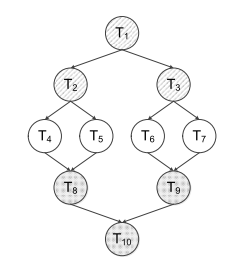
\includegraphics[width=0.5\textwidth]{./dados/figuras/mergesort}
    \fonte{\citeonline{pinto2013escalonamento}}
    \label{fig:figura-mergesort}
\end{figure}

A \autoref{fig:figura-mergesort} demonstra um grafo de dependência de tarefas de um algoritmo de mergesort, nesse exemplo, as tarefas \emph{T1},\emph{T2} e \emph{T3} dividem a entrada inicial, cada uma com metade do tamanho (\emph{n/2}).
Cada metade é uma nova tarefa, sendo que são elas são, \emph{T4}, \emph{T5}, \emph{T6} E \emph{T7}, essas tarefas são responsáveis por ordenar os dados.
Apos isso, as tarefas \emph{T8}, \emph{T9} e \emph{T10} fazem a combinação das partes separadas.

Nesse exemplo é possível notar as dependências de dados que existem entre as tarefas, pois as tarefas de combinação não podem ser executadas antes que as tarefas de divisão e ordenação tenham sido concluídas.

Aplicações baseadas no paradigma de paralelismo de tarefas podem explorar mais os recursos computacionais quando direcionadas a um ambiente de execução.
Após o desenvolvedor descrever as tarefas e as suas dependências, o ambiente é responsável pelo agendamento de tarefas, transferência de dados e gerenciamento das dependências \cite{pinto2017visual}.

Para executar essas atividades descritas acima, o sistema de execução infere características sobre o código da aplicação, como a quantidade de tarefas implementadas, unidade de processamento disponível (quantidade de núcleos de CPU e de dispositivos de GPUs), duração estimada da tarefa, localidade dos dados e largura de interconexão.
Apos isso, o tempo de execução pode usar heurísticas de agendamento apropriadas e executar otimizações para obter um melhor desempenho \cite{pinto2017visual}.

\subsection{StarPU}
StarPU é um sistema de tempo de execução que oferece suporte a arquiteturas multicore heterogêneas, oferecendo uma visão unificada dos recursos computacionais (CPUs e aceleradores ao mesmo tempo).
O ambiente implementa mecanismos para escalonar de forma eficiente as tarefas em uma arquitetura heterogênea \cite{augonnet2011scheduling}. 

Esta ferramenta tem como objetivo permitir que os programadores explorem o poder de computação das CPUs e GPUs disponíveis, ao mesmo tempo que os libera da necessidade de adaptar especialmente seus programas à máquina de destino e unidades de processamento.
StarPU é uma extensão para linguagens da família C (C \textit{Extensions}), ela fornece uma API para descrever as tarefas e as suas dependências que podem existir em uma aplicação \cite{augonnet2011scheduling}.

\newpage

O modelo de execução do StarPU, pode ser descrito por \citeonline{pinto2011ambientes}:
% Pinto (2011):

\begin{citacao}
O modelo de execução do StarPU propõe uma abordagem de tarefas independente da arquitetura base.
São definidos codelets como uma abstração de uma tarefa que pode ser executada em um núcleo de uma CPU multicore ou submetido a um acelerador.
Cada codelet pode ter múltiplas implementações, uma para cada arquitetura em que o codelet pode ser executado.
Cada implementação utiliza as linguagens de programação ou bibliotecas específicas para a arquitetura alvo.
Um codelet contém uma descrição dos dados e o tipo de acesso (leitura, escrita ou ambos).
Codelets são lançados de forma assíncrona. Com isso o escalonador pode reordenar as tarefas para melhorar o desempenho respeitando as dependências entre elas.
Uma aplicação StarPU é descrita como um conjunto de codelets com suas dependências de dados. \cite[p.~26]{pinto2011ambientes}
\end{citacao}

\section{Simulação de Transferência de Calor}